\documentclass{article}
\usepackage[utf8]{inputenc}
\usepackage[none]{hyphenat}
\usepackage[a4paper, total={7in, 8.5in}]{geometry}
\usepackage{graphicx}
\usepackage{amsmath}
\usepackage{amssymb}
\usepackage{mathtools}
\usepackage{bbm}
\usepackage{amsthm}
\usepackage{mathdots}
\usepackage{fancyhdr}
\usepackage[parfill]{parskip}
\usepackage{tikz}
\usepackage{subcaption}
\usepackage{hyperref}
\usepackage{minted}
\theoremstyle{definition}
\newtheorem{theorem}{Theorem}
\newtheorem{definition}{Definition}
\newtheorem{example}{Example}
\newenvironment{theoremqed}
    {\begin{theorem}}
    {\hfill \qedsymbol \end{theorem}}
\newenvironment{definitionqed}
    {\begin{definition}}
    {\hfill \qedsymbol \end{definition}}
\newenvironment{exampleqed}
    {\begin{example}}
    {\hfill \qedsymbol \end{example}}

\renewcommand{\sectionmark}[1]{\markboth{#1}{}}

\renewcommand{\qedsymbol}{\(\blacksquare\)}
\newcommand{\X}{\mathbf{X}}
\renewcommand{\P}{\mathbb{P}}

\setlength{\parskip}{2mm}

\begin{document}

\pagestyle{fancy}
\fancyhead[L]{STA410}
\fancyhead[C]{\nouppercase{\leftmark}}
\fancyhead[R]{Johnny Meng}

\begin{titlepage}
    \centering
    \vspace*{3cm}
    {\huge \bfseries Bayesian Network with Discrete Random Variables and its Python Implementation \par}
    \vspace{5cm}
    {\Large Yuwei (Johnny) Meng \par}
    \vspace{3cm}
    {\large Department of Statistical Sciences, University of Toronto}
    \vfill
\end{titlepage}

\tableofcontents

\pagebreak

\section{Preface \& Acknowledgements}

One day before class, I was talking with Jae and Liam, two other students in STA410, about coming up with a cool name for our Python packages, and I was like ``Oh man I hate coming up with names!'' I do think that cool package names are good, and I admire people coming up with names like \texttt{PyTorch} and \texttt{Beautiful Soup} (when I first learned to use \texttt{Beautiful Soup} I was very confused how this is an HTML parsing library). But yeah, coming up with names doesn't work for me. Just \texttt{BayesNetwork}, or \texttt{BayesianNetwork}. It's cool. It's straightforward. No need to ponder on why \texttt{Beautiful Soup} is for HTML.

Bayesian Network, a variational model for exact inference. The first time I familiarized with this concept was in CSC384, and I thought that this model seems very versatile and powerful. The exposure to the D-Separation, Variable Elimination, and Viterbi algorithms in this course kept my interest in this model. Upon finishing CSC384, I never thought that I would encounter this concept again in CSC412, presented in a more theoretical and mathematical way. What's more, for the third time I was taught Hidden Markov Model in STA410, and I just can't throw this concept out of my mind now. Well, it's something that interests me, so I quickly chose this model to do as my STA410 project.

Here I would like to express my sincere gratitude to \textbf{Professor Alice Gao in CSC384} for introducing Bayesian Network to me in a very entertaining way, to \textbf{Professor Denys Linkov/Murat Erdogdu in CSC412/STA414} for incorporating theories of this model into the course, and definitely to \textbf{Professor Scott Schwartz in STA410} for providing this project opportunity to me to have this model implemented in Python.

\copyright \ Copyright 2025 Johnny Meng

\pagebreak

\section{Bayesian Network}

\subsection{Motivation}

Consider a set of random variables \(\X = (X_1, \cdots, X_n)\) where each \(X_i\in \{x_i, \neg x_i\}\) is binary. To specify the joint distribution of \(\X\), we need to list out all the possible combinations:
\begin{align*}
    &\P(x_1, x_2, \cdots, x_n); \\
    &\P(\neg x_1, x_2, \cdots, x_n); \\
    &\P(x_1, \neg x_2, \cdots, x_n); \\
    &\vdots
\end{align*}
For \(n\) random variables, the number of joint probabilities is \(2^n - 1\), which quickly becomes intractable as \(n\) grows large, requiring a more efficient framework for modeling joint probabilities. Bayesian Network, or Directed Acyclic Graphical Model (DAGM), is one such framework exploiting \textit{Theorem \ref{thm:chain_rule}} below.

\begin{theoremqed} \label{thm:chain_rule}
    \textbf{(Chain Rule of Probability)} Let \(X_1, \cdots, X_n\) be random variables. Then the joint probability can be expressed as
    \begin{align*}
        \P(X_1, \cdots, X_n) &= \P(X_1) \P(X_2, X_3, \cdots, X_n | X_1) \\
        &= \P(X_1) \P(X_2 | X_1) \P(X_3, \cdots, X_n | X_1, X_2) \\
        &= \cdots \\
        &= \P(X_1) \P(X_2 | X_1) \P(X_3 | X_1, X_2) \cdots \P(X_n | X_1, X_2, \cdots, X_{n-1}) \\
        &= \prod_{i=1}^n \P(X_i | X_1, X_2, \cdots, X_{i-1}).
    \end{align*}
\end{theoremqed}

Thus, if we have prior knowledge about the conditional independence relationships between the random variables we are modeling, then we can express the joint distribution in a more compact form, which motivates the use of Bayesian Networks.

\subsection{Introduction to Bayesian Network}

An example of Bayesian Network is shown in \textit{Figure \ref{fig:bayesian_network}} below.

\begin{figure}[htbp]
    \centering
    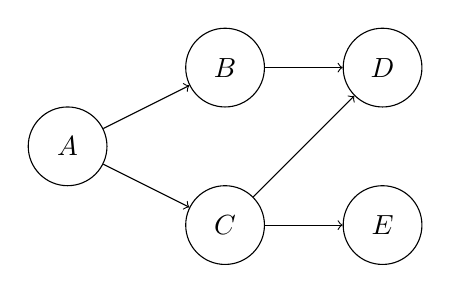
\begin{tikzpicture}
        \node[circle, draw, minimum size=1cm] (A) at (0,0) {\(A\)};
        \node[circle, draw, minimum size=1cm] (B) at (2,1) {\(B\)};
        \node[circle, draw, minimum size=1cm] (C) at (2,-1) {\(C\)};
        \node[circle, draw, minimum size=1cm] (D) at (4,1) {\(D\)};
        \node[circle, draw, minimum size=1cm] (E) at (4,-1) {\(E\)};

        \draw[->] (A) -- (B);
        \draw[->] (A) -- (C);
        \draw[->] (B) -- (D);
        \draw[->] (C) -- (D);
        \draw[->] (C) -- (E);
    \end{tikzpicture}
    \caption{Bayesian Network Example}
    \label{fig:bayesian_network}
\end{figure}

In this Bayesian Network, each vertex represents a random variable. The arrows denote conditional dependencies between random variables. For example, the edge \(A \longrightarrow B\) implies that \(B\) is directly conditionally dependent on \(A\). With this structure, we can model the joint distribution of these random variables in the following way:

\begin{definitionqed} \label{def:bayesian_network}
    Let \(\X = (X_1, \cdots, X_n)\) be a set of random variables modeled by a Bayesian Network. Then the joint probability can be expressed as
    \[\P(X_1, \cdots, X_n) = \prod_{i=1}^n \P(X_i | \operatorname{Parents}(X_i)).\]
\end{definitionqed}

\begin{exampleqed} \label{ex:bayesian_network}
    For the Bayesian Network shown in \textit{Figure \ref{fig:bayesian_network}}, the joint probability can be expressed as
    \[\P(A, B, C, D, E) = \P(A)\cdot\P(B|A)\cdot\P(C|A)\cdot\P(D|B,C)\cdot\P(E|C).\]
\end{exampleqed}

Note that \textit{Definition \ref{def:bayesian_network}} is a special case of \textit{Theorem \ref{thm:chain_rule}}, given that we have prior knowledge of the conditional independence relationships between the random variables. As a result, we can reduce the number of conditionals in the product and express the joint distribution in a more compact form. To illustrate this concept more clearly, let's define some probabilities for the Bayesian Network shown in \textit{Figure \ref{fig:bayesian_network}}. These probabilities will be used throughout the rest of this document.

\begin{exampleqed}
    Let \(A, B, C, D, E \in \{0, 1\}\) be binary random variables with the following conditional probabilities:

    \begin{figure}[htbp]
        \centering
        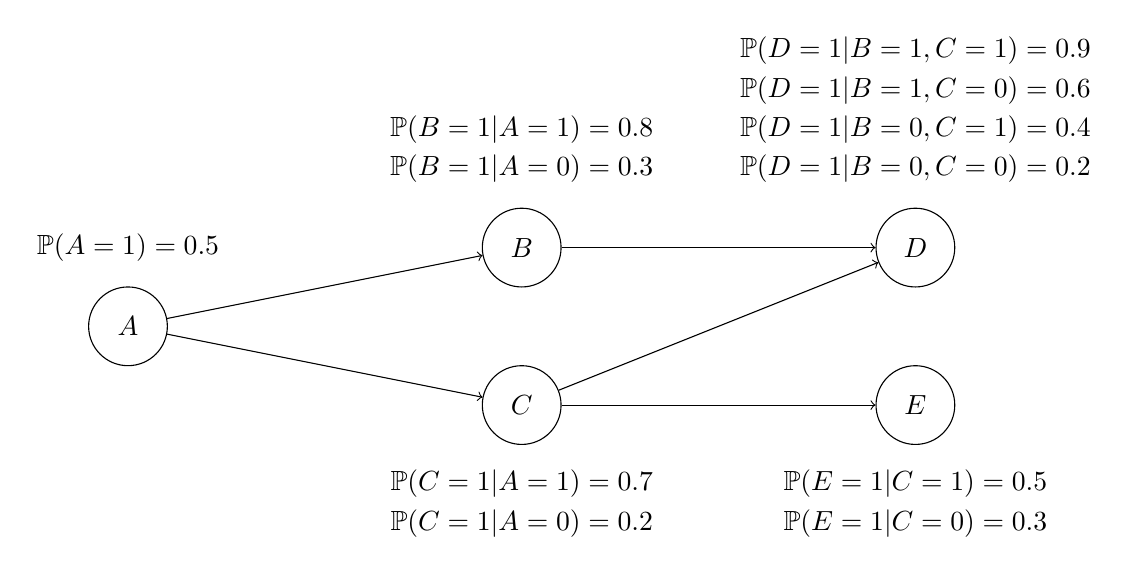
\begin{tikzpicture}
            \node[circle, draw, minimum size=1cm] (A) at (0,0) {\(A\)};
            \node[circle, draw, minimum size=1cm] (B) at (5,1) {\(B\)};
            \node[circle, draw, minimum size=1cm] (C) at (5,-1) {\(C\)};
            \node[circle, draw, minimum size=1cm] (D) at (10,1) {\(D\)};
            \node[circle, draw, minimum size=1cm] (E) at (10,-1) {\(E\)};
    
            \node (P_A) at (0,1) {\(\P(A=1)=0.5\)};
            \node (P_B_A1) at (5,2.5) {\(\P(B=1|A=1)=0.8\)};
            \node (P_B_A0) at (5,2) {\(\P(B=1|A=0)=0.3\)};
            \node (P_C_A1) at (5,-2) {\(\P(C=1|A=1)=0.7\)};
            \node (P_C_A0) at (5,-2.5) {\(\P(C=1|A=0)=0.2\)};
            \node (P_D_B1_C1) at (10,3.5) {\(\P(D=1|B=1,C=1)=0.9\)};
            \node (P_D_B1_C0) at (10,3) {\(\P(D=1|B=1,C=0)=0.6\)};
            \node (P_D_B0_C1) at (10,2.5) {\(\P(D=1|B=0,C=1)=0.4\)};
            \node (P_D_B0_C0) at (10,2) {\(\P(D=1|B=0,C=0)=0.2\)};
            \node (P_E_C1) at (10,-2) {\(\P(E=1|C=1)=0.5\)};
            \node (P_E_C0) at (10,-2.5) {\(\P(E=1|C=0)=0.3\)};
    
            \draw[->] (A) -- (B);
            \draw[->] (A) -- (C);
            \draw[->] (B) -- (D);
            \draw[->] (C) -- (D);
            \draw[->] (C) -- (E);
        \end{tikzpicture}
        \caption{Bayesian Network with Probabilities Example}
        \label{fig:bayesian_network_probs}
    \end{figure}
\end{exampleqed}

Note that only 11 conditional probabilities are needed to specify the joint distribution of the 5 random variables in our Bayesian Network, which is a significant improvement compared to the \(2^5 - 1 = 31\) joint probabilities in the general case. The exact number of required conditional probabilities depends on the structure of the Bayesian Network, though, but as long as there are some conditional independence relationships between the random variables, we can always expect a reduction in the number of required conditional probabilities.

\subsection{Implementation} \label{sec:bn_implementation}

The implementation of Bayesian Network in this project consists of multiple modules which are discussed separately in the following subsections.

\subsubsection{\texttt{Distribution}}

The \texttt{distribution.py} file defines an abstract class called \texttt{Distribution}, as well as two inherited classes named \texttt{UnconditionalDistribution} and \texttt{ConditionalDistribution}. The purpose of these classes is to provide a data structure that encodes the probability distribution of a vertex in the Bayesian Network.

The abstract class \texttt{Distribution} has the attribute and method definitions:

\begin{minted}{python}
    domain: set
\end{minted}

This attribute defines the set of possible values for the random variables.

\begin{minted}{python}
    __call__(self, *args) -> float
\end{minted}

This method evaluates the probability of the random variable taking on a specific value in the domain.

\subsubsection{\texttt{UnconditionalDistribution}}

The \texttt{UnconditionalDistribution} class defines the distribution of a random variable that does not have a parent in the Bayesian Network, as well as the distribution of a random variable conditioned on its parents. Besides the inherited attribute \texttt{domain}, it has the following attribute:

\begin{minted}{python}
    distribution: dict[Any, float]
\end{minted}

This attribute serves as a lookup table for the unconditional distribution of the random variable. The keys of the dictionary are the possible values of the random variable, and the values are the corresponding probabilities.

\begin{minted}{python}
    __init__(self, domain: set, distribution: dict[Any, float]) -> None
\end{minted}

This is the constructor of the class. It takes in the domain and the distribution as arguments. The constructor checks if the provided domain and distribution are valid. If \texttt{domain} does not match the keys of \texttt{distribution}, or the probabilities in \texttt{distribution} do not sum to 1, a \texttt{ValueError} will be raised.

This class also implements the \texttt{\_\_call\_\_} method. The expected argument is a value in the domain of the random variable, and the method outputs the probability of the random variable taking on that value. If the argument is not in the domain, a \texttt{ValueError} will be raised.

\begin{exampleqed}
    For the Bayesian Network shown in \textit{Figure \ref{fig:bayesian_network_probs}}, the distribution of vertex \(A\) would have the following behaviors:

    \begin{minted}{python}
        >>> dist_A = UnconditionalDistribution(domain={0, 1}, distribution={0: 0.5, 1: 0.5})
        >>> dist_A(0)
        0.5
        >>> dist_A(1)
        0.5
    \end{minted}
\end{exampleqed}

\subsubsection{\texttt{ConditionalDistribution}}

This class defines the distribution of a random variable that has parents in the Bayesian Network. It inherits the \texttt{domain} attribute from the \texttt{Distribution} class, and it has the following attributes:

\begin{minted}{python}
    distributions[frozenset[str], UnconditionalDistribution]
\end{minted}

The keys of this dictionary are \texttt{frozenset}s of conditionals of the random variable, and the values define the distribution of the random variable conditioned on the values of its parents.

\begin{minted}{python}
    __init__(self,
             domain: set,
             distributions: dict[frozenset[str], UnconditionalDistribution]) -> None
\end{minted}

This constructor takes in the domain and the distributions as arguments. The constructor checks if the provided domain and distributions are valid. If \texttt{domain} does not match the domain of each \texttt{UnconditionalDistribution} object in \texttt{distribution}, a \texttt{ValueError} will be raised.

This class also implements the \texttt{\_\_call\_\_} method. The expected arguments are a value in the domain of the random variable and a dictionary of the values of its parents. The method outputs the probability of the random variable taking on that value, given the values of its parents. If the value is not in the domain, or if the parents are not in the dictionary, or if the conditioning values are not in the domain of the parents, a \texttt{ValueError} will be raised.

This is slightly confusing, so the following example illustrates this concept.

\begin{exampleqed}
    For the Bayesian Network shown in \textit{Figure \ref{fig:bayesian_network_probs}}, the distribution of vertex \(D\) would have the following behaviors:

    \begin{minted}{python}
        >>> dist_D_B1C1 = UnconditionalDistribution(domain={0, 1}, distribution={0: 0.1, 1: 0.9})
        >>> dist_D_B1C0 = UnconditionalDistribution(domain={0, 1}, distribution={0: 0.4, 1: 0.6})
        >>> dist_D_B0C1 = UnconditionalDistribution(domain={0, 1}, distribution={0: 0.6, 1: 0.4})
        >>> dist_D_B0C0 = UnconditionalDistribution(domain={0, 1}, distribution={0: 0.8, 1: 0.2})
        >>> dist_D = ConditionalDistribution(domain={0, 1}, distributions={
            frozenset({'B: 1', 'C: 1'}): dist_D_B1C1,
            frozenset({'B: 1', 'C: 0'}): dist_D_B1C0,
            frozenset({'B: 0', 'C: 1'}): dist_D_B0C1,
            frozenset({'B: 0', 'C: 0'}): dist_D_B0C0
        })
        >>> dist_D(1, {'B': 1, 'C': 0})
        0.6
        >>> dist_D(0, {'C': 0, 'B': 0})
        0.8
    \end{minted}
\end{exampleqed}

The use of a \texttt{frozenset} data structure is a compromise to the need for a hashable data structure. The advantage is that we don't need to memorize the order of the parents when we are looking up the distribution because there is no inherent order for a \texttt{set} object. When looking up probabilities, the order in which we pass in the parents thus does not matter, as long as the values are correct, which ensures the efficiency of the lookup process.

\subsubsection{\texttt{Vertex}}

The \texttt{Vertex} class represents a vertex in the Bayesian Network. It has the following attributes:

\begin{minted}{python}
    name: str
\end{minted}

This attribute defines the name of the vertex.

\begin{minted}{python}
    domain: set
\end{minted}

This attribute defines the set of possible values for the random variable.

\begin{minted}{python}
    parents: dict[str, Self]
    children: dict[str, Self]
\end{minted}

These two attributes hold the parents and children of the vertex in the Bayesian Network. The keys of the dictionaries are the names of the vertices, and the values are the corresponding \texttt{Vertex} objects.

\begin{minted}{python}
    distribution: Optional[Distribution]
\end{minted}

This attribute holds the distribution of the vertex. Depending on whether the vertex has parents or not, this attribute can be either an \texttt{UnconditionalDistribution} or a \texttt{ConditionalDistribution} object.

The \texttt{Vertex} class also implements the following methods:

\begin{minted}{python}
    __init__(self, name: str, domain: set) -> None
\end{minted}

This constructor takes in the name and domain of the vertex as arguments. It initializes the \texttt{parents}, \texttt{children}, and \texttt{distribution} attributes to empty dictionaries or \texttt{None}.

\begin{minted}{python}
    add_parent(self, parent: Self) -> None
    add_child(self, child: Self) -> None
\end{minted}

These two methods add a parent or child to the vertex. If the added vertex is already a parent or child of the vertex, a \texttt{ValueError} will be raised.

\begin{minted}{python}
    in_domain(self, value: Any) -> bool
\end{minted}

This method returns \texttt{True} if the value is in the domain of the vertex, and \texttt{False} otherwise.

\begin{minted}{python}
    set_distribution(self, distribution: Distribution) -> None
\end{minted}

This method sets the distribution of the vertex. This method contains many checks to ensure that \texttt{distribution} is valid. If \texttt{distribution} is not compatible with the vertex, a \texttt{ValueError} will be raised.

\begin{minted}{python}
    __call__(self, *args) -> float
\end{minted}

This method basically calls the \texttt{\_\_call\_\_} method of the \texttt{distribution} object with the arguments \texttt{*args}. The expected arguments are the same as the \texttt{\_\_call\_\_} method of the \texttt{distribution} object and outputs a probability. If the \texttt{distribution} attribute for the vertex is \texttt{None}, a \texttt{ValueError} will be raised.

\subsubsection{\texttt{BayesNetwork}}

This class represents the Bayesian Network. It has the following attribute:

\begin{minted}{python}
    vertices: dict[str, Vertex]
\end{minted}

This attribute holds a list of the vertices in the Bayesian Network. The keys of the dictionary are the names of the vertices, and the values are the corresponding \texttt{Vertex} objects.

The \texttt{BayesNetwork} class implements the following methods:

\begin{minted}{python}
    __init__(self) -> None
\end{minted}

The constructor creates a \texttt{BayesNetwork} object and initializes the \texttt{vertices} attribute to an empty dictionary.

\begin{minted}{python}
    __len__(self) -> int
\end{minted}

This method returns the number of vertices in the Bayesian Network.

\begin{minted}{python}
    add_node(self, vertex: Vertex) -> None
\end{minted}

This method adds a vertex to the Bayesian Network. If the vertex is already in the network, a \texttt{ValueError} will be raised.

\begin{minted}{python}
    add_edge(self, parent: Vertex, child: Vertex) -> None
\end{minted}

This method adds an edge from the parent vertex to the child vertex in the Bayesian Network. If either vertex is not in the network, a \texttt{ValueError} will be raised.

\begin{minted}{python}
    find_roots(self) -> list[Vertex]
\end{minted}

This method returns a list of the root vertices in the Bayesian Network. A root vertex is defined as a vertex that does not have any parents in the network.

\begin{minted}{python}
    __call__(self, *args) -> float
\end{minted}

This method evaluates the joint probability of the random variables in the Bayesian Network. The expected argument is a dictionary with the keys being the names of the random variables and the values being the corresponding values. The method outputs the joint probability of the random variables taking on those values. If values for one or more random variables are not provided, a \texttt{ValueError} will be raised. To compute the probability of a subset of the random variables, use the \textit{Variable Elimination} algorithm discussed in \textit{Chapter \ref{sec:variable_elimination}}

\subsubsection{\texttt{read\_bayes\_network\_from\_txt}}

The above description might be very confusing, so it is not recommended to create a Bayesian Network from scratch. Instead, I provide a function to read in a Bayesian Network from a text file. An example of this text file is provided in this \href{https://github.com/BullDF/bayes_network/blob/main/bn_ex.txt}{\texttt{bn\_ex.txt}} file. The text file requires 3 parts, explained using the example file and \textit{Figure \ref{fig:bayesian_network_probs}}:

\begin{verbatim}
    A: {0, 1}
    B: {0, 1}
    C: {0, 1}
    D: {0, 1}
    E: {0, 1}
\end{verbatim}

This part defines the vertices in the Bayesian Network. Each line contains the name of the vertex and its domain, enclosed in curly braces. The vertices are separated by new lines.

\begin{verbatim}
    A -> B
    A -> C
    B -> D
    C -> D
    C -> E
\end{verbatim}

This part defines the edges in the Bayesian Network. Each line contains the name of the parent vertex and the name of the child vertex, separated by an arrow (\texttt{->}). The edges are separated by new lines.

\begin{verbatim}
    P(A = 1) = 0.5
    P(A = 0) = 0.5

    P(B = 1 | A = 1) = 0.8
    P(B = 0 | A = 1) = 0.2
    P(B = 1 | A = 0) = 0.3
    P(B = 0 | A = 0) = 0.7

    P(D = 1 | B = 1, C = 1) = 0.9
    P(D = 0 | B = 1, C = 1) = 0.1
    P(D = 1 | B = 1, C = 0) = 0.6
    P(D = 0 | B = 1, C = 0) = 0.4
    P(D = 1 | B = 0, C = 1) = 0.4
    P(D = 0 | B = 0, C = 1) = 0.6
    P(D = 1 | B = 0, C = 0) = 0.2
    P(D = 0 | B = 0, C = 0) = 0.8
    
    ...
\end{verbatim}

This part defines the unconditional and conditional distributions of the vertices in the Bayesian Network. The conditional distributions are separated by new lines. Note that it is necessary to provide the probabilities for both \texttt{P(A = 1)} and \texttt{P(A = 0)} in the text file, even though the complement can be easily computed.

As long as the format is followed, the order in which the vertices, edges, and distributions are defined does not matter because the function uses regular expression to parse the text file. The function will create a \texttt{BayesNetwork} object and add the vertices, edges, and distributions to the object. The function then returns the \texttt{BayesNetwork} object. It is strongly recommended to use this function to create a Bayesian Network.

To wrap up this section, below is an example of how to use the function to create a Bayesian Network from a text file.

\begin{exampleqed}
    Assume that the text file is named \texttt{\texttt{bn\_ex.txt}} and is in the same directory as the Python file.

    \begin{minted}{python}
        >>> bn = read_bayes_network_from_txt('bn_ex.txt')
        >>> bn.find_roots()
        [A: {0, 1}]
        >>> len(bn)
        5
    \end{minted}

    Regarding joint probability computations:
    \begin{align*}
        \P(A=1, B=0, C=1, D=1, E=0) &= \P(A=1)\P(B=0|A=1)\P(C=1|A=1)\P(D=1|B=0,C=1) \\
        &\quad \cdot \P(E=0|C=1) \\
        &= 0.5 \cdot 0.2 \cdot 0.7 \cdot 0.4 \cdot 0.5 \\
        &= 0.014.
    \end{align*}

    The code output confirms this result:

    \begin{minted}{python}
        >>> bn({'A': 1, 'B': 0, 'C': 1, 'D': 1, 'E': 0})
        0.013999999999999999 # Numerical roundoff error
    \end{minted}
\end{exampleqed}

\pagebreak

\section{Variable Elimination} \label{sec:variable_elimination}

\subsection{Motivation}

In the previous section, we introduced how we could easily compute the joint probability of the random variables in a Bayesian Network. However, \textit{Definition \ref{def:bayesian_network}} must be used when the joint probability involves all random variables in the network and cannot be applied when we want to calculate the joint probability of a subset of the random variables or a conditional probability of the random variables. This motivates the use of the \textit{Variable Elimination} algorithm.

Below is the example Bayesian Network again for reference:
\begin{figure}[htbp]
    \centering
    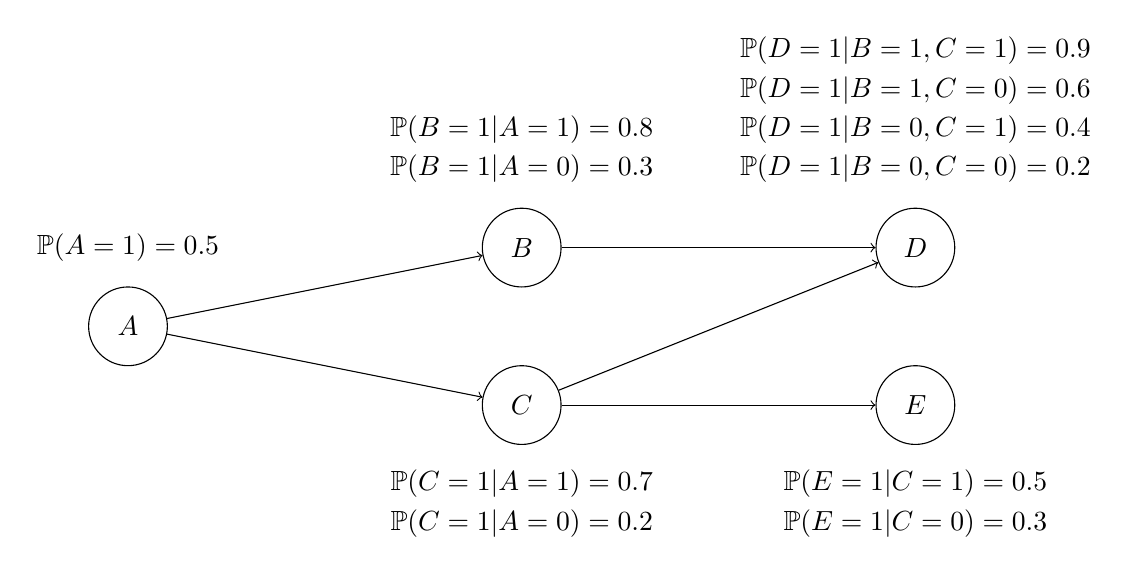
\begin{tikzpicture}
        \node[circle, draw, minimum size=1cm] (A) at (0,0) {\(A\)};
        \node[circle, draw, minimum size=1cm] (B) at (5,1) {\(B\)};
        \node[circle, draw, minimum size=1cm] (C) at (5,-1) {\(C\)};
        \node[circle, draw, minimum size=1cm] (D) at (10,1) {\(D\)};
        \node[circle, draw, minimum size=1cm] (E) at (10,-1) {\(E\)};

        \node (P_A) at (0,1) {\(\P(A=1)=0.5\)};
        \node (P_B_A1) at (5,2.5) {\(\P(B=1|A=1)=0.8\)};
        \node (P_B_A0) at (5,2) {\(\P(B=1|A=0)=0.3\)};
        \node (P_C_A1) at (5,-2) {\(\P(C=1|A=1)=0.7\)};
        \node (P_C_A0) at (5,-2.5) {\(\P(C=1|A=0)=0.2\)};
        \node (P_D_B1_C1) at (10,3.5) {\(\P(D=1|B=1,C=1)=0.9\)};
        \node (P_D_B1_C0) at (10,3) {\(\P(D=1|B=1,C=0)=0.6\)};
        \node (P_D_B0_C1) at (10,2.5) {\(\P(D=1|B=0,C=1)=0.4\)};
        \node (P_D_B0_C0) at (10,2) {\(\P(D=1|B=0,C=0)=0.2\)};
        \node (P_E_C1) at (10,-2) {\(\P(E=1|C=1)=0.5\)};
        \node (P_E_C0) at (10,-2.5) {\(\P(E=1|C=0)=0.3\)};

        \draw[->] (A) -- (B);
        \draw[->] (A) -- (C);
        \draw[->] (B) -- (D);
        \draw[->] (C) -- (D);
        \draw[->] (C) -- (E);
    \end{tikzpicture}
    \caption{Bayesian Network with Probabilities Example}
    \label{fig:bayesian_network_probs_vea}
\end{figure}

Some examples of probabilities we might want to compute are as follows:
\begin{align*}
    &\P(A, B, C, D); \\
    &\P(B, C | D); \\
    &\P(B, E | A); \\
    &\P(A, B | C, D); \\
    &\P(E); \\
    &\vdots
\end{align*}

With the \textit{Variable Elimination} algorithm, these probabilities can be computed easily.

\subsection{Theory}

The \textit{Variable Elimination} algorithm is based on the following theorem:

\begin{theoremqed} \label{thm:marginal}
    \textbf{(Marginal Probability)} Given discrete random variables \(X, Y\), the marginal probabilities can be computed as
    \begin{align*}
        p_X(x) &= \sum_y p_{XY}(x, y) \\
        &= \sum_y p_{X|Y}(x|y) p_Y(y); \\
        p_Y(y) &= \sum_x p_{XY}(x, y) \\
        &= \sum_x p_{Y|X}(y|x) p_X(x).
    \end{align*}
\end{theoremqed}

With \textit{Theorem \ref{thm:marginal}}, the \textit{Variable Elimination} algorithm is as follows:

\begin{theoremqed} \label{thm:vea}
    \textbf{(Variable Elimination Algorithm)} Given a Bayesian Network with vertices \(\X = \{X_1, \cdots, X_n\}\) and a desired probability \(\P(Q | E)\) with \(Q \subseteq \X\), \(E \subseteq \X\), \(Q \cap E = \varnothing\), define \(H = \X \setminus Q \cup E\) as the hidden variables. Let \(D_X\) denote the domain of random variable \(X\). Then
    \[\P(Q | E) = \operatorname{normalize}\left(\sum_{X_h \in H} \sum_{x\in D_{X_h}} \prod_{\psi \in \mathcal{F}} \psi(X_h|E) \right),\]
    where the notation \(\psi(X_h|E)\) denotes the ``factor'' that concerns the hidden variable \(X_h\) conditioned on \(E\), and \(\mathcal{F}\) defines the set of all the ``factors''.
\end{theoremqed}

\textit{Theorem \ref{thm:vea}} defines some new concepts such as \textit{hidden variables} and \textit{factors} that might be confusing, so I devote the following section to give an example of using the \textit{Variable Elimination} algorithm to compute a probability.

\subsection{Example}

Given Bayesian Network \textit{Figure \ref{fig:bayesian_network_probs_vea}}, suppose we want to compute conditional probability
\[\P(A, E | D = 0).\]

\subsubsection{Step I -- Creating Initial Factors}

For each node in the Bayesian Network, we create a factor consisting of its probabilities defined by the network. Each factor has a scope denoting the set of random variables it concerns. For the Bayesian Network in \textit{Figure \ref{fig:bayesian_network_probs_vea}}, we would create the following initial factors:
\begin{align*}
    f_1(A) &= \begin{pmatrix}
        A = 1 & 0.5 \\
        A = 0 & 0.5
    \end{pmatrix} \\
    f_2(A, B) &= \begin{pmatrix}
        A = 1 & B = 1 & 0.8 \\
        A = 1 & B = 0 & 0.2 \\
        A = 0 & B = 1 & 0.3 \\
        A = 0 & B = 0 & 0.7
    \end{pmatrix} \\
    f_3(A, C) &= \begin{pmatrix}
        A = 1 & C = 1 & 0.7 \\
        A = 1 & C = 0 & 0.3 \\
        A = 0 & C = 1 & 0.2 \\
        A = 0 & C = 0 & 0.8
    \end{pmatrix}
    \intertext{}
    f_4(B, C, D) &= \begin{pmatrix}
        B = 1 & C = 1 & D = 1 & 0.9 \\
        B = 1 & C = 1 & D = 0 & 0.1 \\
        B = 1 & C = 0 & D = 1 & 0.6 \\
        B = 1 & C = 0 & D = 0 & 0.4 \\
        B = 0 & C = 1 & D = 1 & 0.4 \\
        B = 0 & C = 1 & D = 0 & 0.6 \\
        B = 0 & C = 0 & D = 1 & 0.2 \\
        B = 0 & C = 0 & D = 0 & 0.8
    \end{pmatrix} \\
    f_5(C, E) &= \begin{pmatrix}
        C = 1 & E = 1 & 0.5 \\
        C = 1 & E = 0 & 0.5 \\
        C = 0 & E = 1 & 0.3 \\
        C = 0 & E = 0 & 0.7
    \end{pmatrix}
\end{align*}

Note that whether the probabilities are conditional or not do not matter in the factors. The factors only care about the random variables they concern. As a reference, the set of factors we have after step 1 is
\[\mathcal{F}_1 = \{f_1, f_2, f_3, f_4, f_5\}.\]

\subsubsection{Step II -- Restricting Evidence}

The evidence we have is \(D = 0\), and so we can discard entries of \(D\) that are irrelevant. Specifically, \(f_4\) turns into
\[f_6(B, C) = \begin{pmatrix}
    B = 1 & C = 1 & 0.1 \\
    B = 1 & C = 0 & 0.4 \\
    B = 0 & C = 1 & 0.6 \\
    B = 0 & C = 0 & 0.8
\end{pmatrix}\]
Note that we can also remove \(D\) from the scope of \(f_4\) because we have restricted it based on the evidence.

After step 2, the set of factors is
\[\mathcal{F}_2 = \{f_1, f_2, f_3, f_5, f_6\}.\]
Note that each factor is used only once and we can safely discard it afterwards.

\subsubsection{Step III -- Eliminating Hidden Variables}

In our probability, \(A, E\) are the \textit{Query} variables because we are interested in their joint probabilities. \(D\) is the \textit{Evidence} variable because we have evidence of it. The remaining variables, \(B\) and \(C\), are \textit{Hidden} variables, and we will be removing them in this step.

The computational complexity of the \textit{Variable Elimination} algorithm is \(O(mk^{N_{\max}})\), where \(m\) is the number of initial factors, \(k\) is the maximum number of values in the domain of the variables, and \(N_{\max}\) is the number of variables inside the largest sum. However, this complexity largely depends on the order in which we eliminate the hidden variables, and finding the optimal order of elimination is \textsf{NP}-hard. For a small Bayesian Network like the one in our case, the order doesn't matter much, so I will predetermine the order to be \(B \to C\).

To eliminate \(B\), we will gather all factors that concern the variable \(B\), in our case they are \(f_2\) and \(f_6\). We will consider every valid combination of the variables and multiply the probability values if the conditions match. After multiplying, we get
\[f_7(A, B, C) = \begin{pmatrix}
    A = 1 & B = 1 & C = 1 & 0.8\cdot 0.1 = 0.08 \\
    A = 1 & B = 1 & C = 0 & 0.8\cdot 0.4 = 0.32 \\
    A = 1 & B = 0 & C = 1 & 0.2\cdot 0.6 = 0.12 \\
    A = 1 & B = 0 & C = 0 & 0.2\cdot 0.8 = 0.16 \\
    A = 0 & B = 1 & C = 1 & 0.3\cdot 0.1 = 0.03 \\
    A = 0 & B = 1 & C = 0 & 0.3\cdot 0.4 = 0.12 \\
    A = 0 & B = 0 & C = 1 & 0.7\cdot 0.6 = 0.42 \\
    A = 0 & B = 0 & C = 0 & 0.7\cdot 0.8 = 0.56
\end{pmatrix}\]
Next, we will sum out \(B\) and obtain
\[f_8(A, C) = \begin{pmatrix}
    A = 1 & C = 1 & 0.08 + 0.12 = 0.2 \\
    A = 1 & C = 0 & 0.32 + 0.16 = 0.48 \\
    A = 0 & C = 1 & 0.03 + 0.42 = 0.45 \\
    A = 0 & C = 0 & 0.12 + 0.56 = 0.68
\end{pmatrix}\]
Now we have eliminated variable \(B\). As a reference, the set of factors we have after this step is
\[\mathcal{F}_3 = \{f_1, f_3, f_5, f_8\}.\]
We will do the same thing for variable \(C\). We gather factors \(f_3\), \(f_5\) and \(f_8\) that concern \(C\), and we multiply them together:
\[f_9(A, C, E) = \begin{pmatrix}
    A = 1 & C = 1 & E = 1 & 0.7\cdot 0.5 \cdot 0.2 = 0.07 \\
    A = 1 & C = 1 & E = 0 & 0.7\cdot 0.5 \cdot 0.2 = 0.07 \\
    A = 1 & C = 0 & E = 1 & 0.3\cdot 0.3 \cdot 0.48 = 0.0432 \\
    A = 1 & C = 0 & E = 0 & 0.3\cdot 0.7 \cdot 0.48 = 0.1008 \\
    A = 0 & C = 1 & E = 1 & 0.2\cdot 0.5 \cdot 0.45 = 0.045 \\
    A = 0 & C = 1 & E = 0 & 0.2\cdot 0.5 \cdot 0.45 = 0.045 \\
    A = 0 & C = 0 & E = 1 & 0.8\cdot 0.3 \cdot 0.68 = 0.1632 \\
    A = 0 & C = 0 & E = 0 & 0.8\cdot 0.7 \cdot 0.68 = 0.3808
\end{pmatrix}\]
Then, we sum out \(C\):
\[f_{10}(A, E) = \begin{pmatrix}
    A = 1 & E = 1 & 0.07 + 0.0432 = 0.1132 \\
    A = 1 & E = 0 & 0.07 + 0.1008 = 0.1708 \\
    A = 0 & E = 1 & 0.045 + 0.1632 = 0.2082 \\
    A = 0 & E = 0 & 0.045 + 0.3808 = 0.4258
\end{pmatrix}\]
After this step, the remaining factors are
\[\mathcal{F}_4 = \{f_1, f_{10}\}.\]

\subsubsection{Step IV -- Combining and Normalization}

At this step, all remaining factors should concern only our query variables. We will combine the remaining factors (\(f_1, f_{10}\)) by multiplying them like we did previously:
\[f_{11}(A, E) = \begin{pmatrix}
    A = 1 & E = 1 & 0.5\cdot 0.1132 = 0.0566 \\
    A = 1 & E = 0 & 0.5\cdot 0.1708 = 0.0854 \\
    A = 0 & E = 1 & 0.5\cdot 0.2082 = 0.1041 \\
    A = 0 & E = 0 & 0.5\cdot 0.4258 = 0.2129
\end{pmatrix}\]

We are almost done. We just need to normalize the remaining values so that they follow a probability distribution. The current sum is \(0.0566 + 0.0854 + 0.1041 + 0.2129 = 0.459\). We can normalize the values by dividing each value by the sum, rounded to 3 decimal points:
\[\P(A, E | D = 0) = \begin{pmatrix}
    A = 1 & E = 1 & 0.0566/0.459 = 0.123 \\
    A = 1 & E = 0 & 0.0854/0.459 = 0.186 \\
    A = 0 & E = 1 & 0.1041/0.459 = 0.227 \\
    A = 0 & E = 0 & 0.2129/0.459 = 0.464
\end{pmatrix}\]

\subsection{Implementation}

The \textit{Variable Elimination} algorithm is implemented in the \texttt{variable\_elimination.py} file. Each step mentioned above gets its own helper function, but the entire pipeline can be executed by calling the \texttt{variable\_elimination} function. This function has the following signature:

\begin{minted}{python}
    variable_elimination(bn: BayesNetwork, query: set, evidence: dict={}) -> dict
\end{minted}

Running code for the example illustrated above, we would get the outputs

\begin{minted}{python}
    >>> bn = read_bayes_network_from_txt('bn_ex.txt')
    >>> variable_elimination(bn, query={'A', 'E'}, evidence={'D': 0})
    {{'A: 1', 'E: 1'}: 0.12331154684095862,
     {'E: 1', 'A: 0'}: 0.22679738562091506,
     {'A: 1', 'E: 0'}: 0.18605664488017432,
     {'E: 0', 'A: 0'}: 0.46383442265795205}
\end{minted}

which match our manual calculations above.

\pagebreak

\section{Ancestral Sampling}

A Bayesian Network is nonetheless a model for a set of random variables, and thus we can sample from it. One way to sample from a Bayesian Network is \textit{Ancestral Sampling}. The joint probability formula for a Bayesian Network defined in \textit{Definition \ref{def:bayesian_network}} suggests that we can sample each random variable based on the conditional distribution given its parents in a topological order, which also gives birth to the name \textit{Ancestral Sampling}.

\begin{exampleqed}
    Given the Bayesian Network in \textit{Figure \ref{fig:bayesian_network_probs}}, we can sample from it as follows:
    \begin{enumerate}
        \item Sample the root node \(A\) as a Bernoulli random variable with probability \(\P(A)\);
        \item Sample the next layer of nodes \(B\) and \(C\) conditioned on the sampled value of \(A\) using the conditional distributions \(\P(B|A)\) and \(\P(C|A)\);
        \item Sample the final layer of nodes \(D\) and \(E\) conditioned on the sampled values of \(B\) and \(C\) using the conditional distributions \(\P(D|B,C)\) and \(\P(E|C)\);
        \item The sampled values of \(A, B, C, D, E\) form a sample of the joint distribution of the random variables. Repeat this process to obtain more samples.
    \end{enumerate}
\end{exampleqed}

This method is implemented in the \texttt{ancestral\_sampling.py} file. The function has the following signature:

\begin{minted}{python}
    ancestral_sampling(bn: BayesNetwork, n: int=1) -> Union[dict, list[dict]]
\end{minted}

This function takes in a \texttt{BayesNetwork} instance and the number of samples \(n\), whose default value is 1. The function returns a dictionary containing the sampled values of the random variables. If \(n > 1\), the function returns a list of dictionaries, each representing a sample. Below is an example usage of the function:

\begin{minted}{python}
    >>> bn = read_bayes_network_from_txt('bn_ex.txt')
    >>> ancestral_sampling(bn)
    {'A': 1, 'B': 0, 'C': 1, 'D': 1, 'E': 0}
    >>> ancestral_sampling(bn, n=5)
    [{'A': 0, 'B': 0, 'C': 1, 'D': 1, 'E': 1},
     {'A': 0, 'B': 0, 'C': 0, 'D': 1, 'E': 1},
     {'A': 0, 'B': 0, 'C': 0, 'D': 0, 'E': 0},
     {'A': 1, 'B': 1, 'C': 0, 'D': 1, 'E': 0},
     {'A': 0, 'B': 0, 'C': 1, 'D': 0, 'E': 1}]
\end{minted}

\pagebreak

\section{Hidden Markov Model (HMM)}

\subsection{Introduction to HMM} \label{sec:hmm_intro}

A \textit{Hidden Markov Model}, or an HMM, is a special case of Bayesian Networks. An HMM has only two types of nodes: \textit{Hidden} nodes and \textit{Observation} nodes. In real-world applications, the hidden nodes represent states of a system that are not directly observable, while the observation nodes represent observable events that are generated by the hidden states. For \(t\in \{0, 1, \cdots\}\), let \(Z_t\) denote the hidden state at time \(t\) and \(X_t\) denote the observation at time \(t\). An HMM, as a Bayesian Network, has the following structure:

\begin{figure}[htbp]
    \centering
    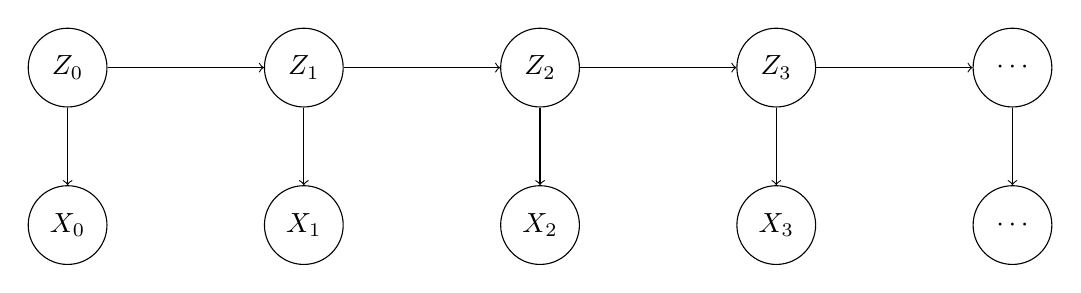
\begin{tikzpicture}
        \node[circle, draw, minimum size=1cm] (Z0) at (0,0) {\(Z_0\)};
        \node[circle, draw, minimum size=1cm] (X0) at (0,-2) {\(X_0\)};
        \node[circle, draw, minimum size=1cm] (Z1) at (3,0) {\(Z_1\)};
        \node[circle, draw, minimum size=1cm] (X1) at (3,-2) {\(X_1\)};
        \node[circle, draw, minimum size=1cm] (Z2) at (6,0) {\(Z_2\)};
        \node[circle, draw, minimum size=1cm] (X2) at (6,-2) {\(X_2\)};
        \node[circle, draw, minimum size=1cm] (Z3) at (9,0) {\(Z_3\)};
        \node[circle, draw, minimum size=1cm] (X3) at (9,-2) {\(X_3\)};
        \node[circle, draw, minimum size=1cm] (Z_inf) at (12,0) {\(\cdots\)};
        \node[circle, draw, minimum size=1cm] (X_inf) at (12,-2) {\(\cdots\)};

        \draw[->] (Z0) -- (Z1);
        \draw[->] (Z1) -- (Z2);
        \draw[->] (Z2) -- (Z3);
        \draw[->] (Z3) -- (Z_inf);
        \draw[->] (Z0) -- (X0);
        \draw[->] (Z1) -- (X1);
        \draw[->] (Z2) -- (X2);
        \draw[->] (Z3) -- (X3);
        \draw[->] (Z_inf) -- (X_inf);
    \end{tikzpicture}
    \caption{Hidden Markov Model Structure}
    \label{fig:hmm_structure}
\end{figure}

Note that an HMM can have infinitely many nodes as \(t \to \infty\). At each time step \(t\), the hidden state \(Z_t\) generates an observation \(X_t\), modeled by the conditional dependence \(Z_t \longrightarrow X_t\). This implies that observation \(X_t\) only depends on the current hidden state \(Z_t\), which is an important property of HMMs. Additionally, note the conditional dependence \(Z_{t-1} \longrightarrow Z_t\), which implies that the hidden state at time \(t\) only depends on the hidden state at time \(t-1\), and not on other hidden or observation states.

Given the HMM in \textit{Figure \ref{fig:hmm_structure}}, from previous sections we know that we can define different distributions for the hidden states and observation states. However, since the time step \(t\) can approach \(\infty\), defining the distributions for all hidden states and observation states separately is impractical. Therefore, we will make an assumption about our HMM here called \textit{stationarity}:

\begin{definitionqed} \label{def:stationarity}
    \textbf{(Stationarity of HMMs)} An HMM is \textit{stationary} if it satisfies the following conditions:
    \begin{enumerate}
        \item \(\P(Z_t | Z_{t-1})\) is the same for every time step \(t\);
        \item \(\P(X_t | Z_t)\) is the same for every time step \(t\).
    \end{enumerate}
\end{definitionqed}

With the assumption defined in \textit{Definition \ref{def:stationarity}}, we only need to define the following three sets of distributions for an HMM, which is much easier to do:

\begin{definitionqed} \label{def:hmm}
    A stationary HMM is specified by the following distributions:
    \begin{enumerate}
        \item \textbf{Initial Distribution} -- \(\pi(i) = \P(Z_0 = i)\). The probability that the initial hidden state is \(i\).
        \item \textbf{Transition Distribution} -- \(\psi(i, j) = \P(Z_t = j | Z_{t-1} = i)\). The probability that the hidden state at time \(t\) is \(j\) given that the hidden state at time \(t-1\) is \(i\).
        \item \textbf{Emission Distribution} -- \(\phi(i, k) = \P(X_t = k | Z_t = i)\). The probability that the observation at time \(t\) is \(k\) given that the hidden state at time \(t\) is \(i\).
    \end{enumerate}
\end{definitionqed}

Similar to \textit{Figure \ref{fig:bayesian_network_probs}} where we defined some probabilities for illustration, we will define the following HMM and use these probabilities for subsequent examples:

\pagebreak

\begin{exampleqed}
    Let \(Z_t \in \{c, h\}\) denote whether the weather is \textit{cold} or \textit{hot} on day \(t\). Let \(X_t \in \{0, 1, 2\}\) denote the number of ice creams you eat on day \(t\). We define the following probability distributions:

    \begin{figure}[htbp]
        \centering
        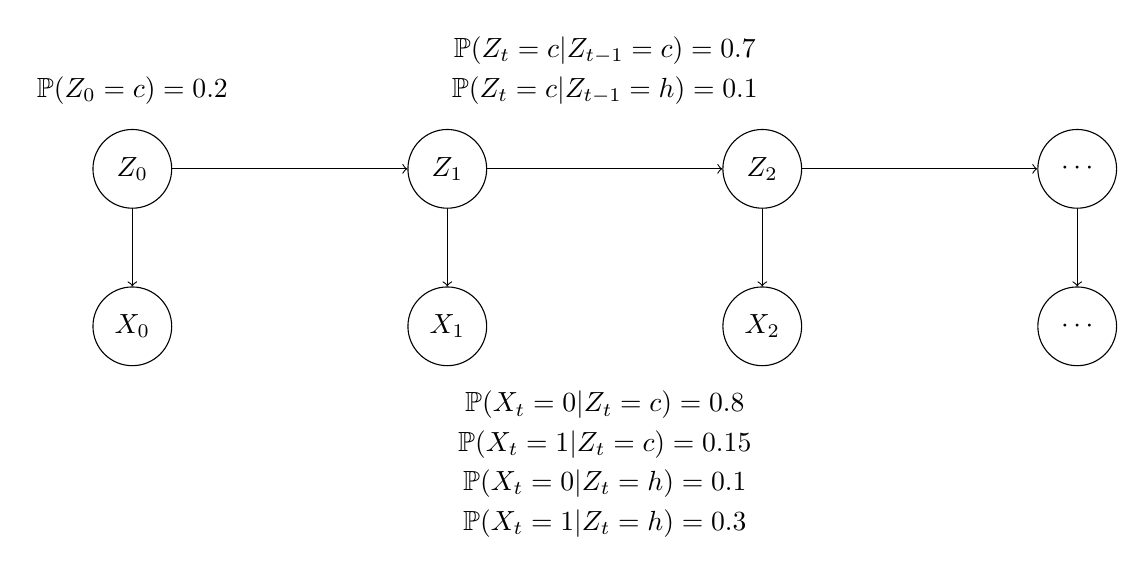
\begin{tikzpicture}
            \node[circle, draw, minimum size=1cm] (Z0) at (0,0) {\(Z_0\)};
            \node[circle, draw, minimum size=1cm] (X0) at (0,-2) {\(X_0\)};
            \node[circle, draw, minimum size=1cm] (Z1) at (4,0) {\(Z_1\)};
            \node[circle, draw, minimum size=1cm] (X1) at (4,-2) {\(X_1\)};
            \node[circle, draw, minimum size=1cm] (Z2) at (8,0) {\(Z_2\)};
            \node[circle, draw, minimum size=1cm] (X2) at (8,-2) {\(X_2\)};
            \node[circle, draw, minimum size=1cm] (Z_inf) at (12,0) {\(\cdots\)};
            \node[circle, draw, minimum size=1cm] (X_inf) at (12,-2) {\(\cdots\)};
    
            \node (P_Z0) at (0,1) {\(\P(Z_0 = c) = 0.2\)};
            \node (P_Z_c) at (6, 1.5) {\(\P(Z_t = c | Z_{t-1} = c) = 0.7\)};
            \node (P_Z_h) at (6, 1) {\(\P(Z_t = c | Z_{t-1} = h) = 0.1\)};
            \node (P_X0_c) at (6, -3) {\(\P(X_t = 0 | Z_t = c) = 0.8\)};
            \node (P_X1_c) at (6, -3.5) {\(\P(X_t = 1 | Z_t = c) = 0.15\)};
            \node (P_X0_h) at (6, -4) {\(\P(X_t = 0 | Z_t = h) = 0.1\)};
            \node (P_X1_h) at (6, -4.5) {\(\P(X_t = 1 | Z_t = h) = 0.3\)};
    
            \draw[->] (Z0) -- (Z1);
            \draw[->] (Z1) -- (Z2);
            \draw[->] (Z2) -- (Z_inf);
            \draw[->] (Z0) -- (X0);
            \draw[->] (Z1) -- (X1);
            \draw[->] (Z2) -- (X2);
            \draw[->] (Z_inf) -- (X_inf);
        \end{tikzpicture}
        \caption{HMM with Probabilities Example}
        \label{fig:hmm_probs}
    \end{figure}
\end{exampleqed}

Besides computing the joint probabilities using \textit{Definition \ref{def:bayesian_network}} or the \hyperref[sec:variable_elimination]{\textit{Variable Elimination}} algorithm on an HMM, given a sequence of observations \(\vec x = [x_0, x_1, \cdots, x_T]\), there are 4 common types of tasks that we can perform with an HMM:

\begin{enumerate}
    \item \textbf{Filtering} -- \(\P(Z_T | \vec x)\). Compute the probability of the hidden state at \textit{current} time \(T\) based on all observations. This can be done using the \textit{Forward} algorithm discussed in \textit{Chapter \ref{sec:forward_algorithm}};
    \item \textbf{Smoothing} -- \(\P(Z_t | \vec x)\) for \(0 \leq t < T\). Compute the probability of the hidden state at \textit{past} time \(t\) based on all observations. This can be done using the \textit{Forward-Backward} algorithm discussed in \textit{Chapter \ref{sec:forward_backward_algorithm}};
    \item \textbf{Prediction} -- \(\P(Z_t | \vec x)\) for \(t > T\). Compute the probability of the hidden state at \textit{future} time \(t\) based on all observations. This is currently not implemented;
    \item \textbf{Most Likely Sequence} -- \(\arg \max_{\vec z} \P(\vec z | \vec x)\). Compute the most likely sequence of hidden states given the observations. This can be done using the \textit{Viterbi} algorithm discussed in \textit{Chapter \ref{sec:viterbi_algorithm}}.
\end{enumerate}

\subsection{Implementation}

\subsubsection{\texttt{HiddenMarkovModel}}

The \texttt{HiddenMarkovModel} class is implemented in the \texttt{hmm.py} file. This class extends the \texttt{BayesNetwork} class discussed in \textit{Chapter \ref{sec:bn_implementation}}, because an HMM is essentially a special type of Bayesian Network. The class has the following attributes:

\begin{minted}{python}
    time_step: Optional[int]
\end{minted}

This attribute stores the number of time steps for the HMM.

\begin{minted}{python}
    hidden_domain: Optional[set]
    observation_domain: Optional[set]
\end{minted}

These two attributes store the domains of the hidden and observation variables, respectively.

\begin{minted}{python}
    initial_distribution: Optional[UnconditionalDistribution]
    transition_distribution: Optional[ConditionalDistribution]
    emission_distribution: Optional[ConditionalDistribution]
\end{minted}

These three attributes define the distributions of the HMM as specified in \textit{Definition \ref{def:hmm}}.

In addition to the methods implemented in \texttt{BayesNetwork} as documented in \textit{Chapter \ref{sec:bn_implementation}}, this class implements the following methods:

\begin{minted}{python}
    __init__(self) -> None
\end{minted}

This constructor initializes a \texttt{HiddenMarkovModel} instance. It takes no arguments and initializes all the attributes to \texttt{None}.

\begin{minted}{python}
    set_time_step(self, time_step: int) -> None
    set_hidden_domain(self, hidden_domain: set) -> None
    set_observation_domain(self, observation_domain: set) -> None
    set_initial_distribution(self, initial_distribution: UnconditionalDistribution) -> None
    set_transition_distribution(self, transition_distribution: ConditionalDistribution) -> None
    set_emission_distribution(self, emission_distribution: ConditionalDistribution) -> None
\end{minted}

These methods basically set the corresponding attributes of the \texttt{HiddenMarkovModel} instance.

\subsubsection{\texttt{read\_hmm\_from\_txt}}

Similar to \texttt{BayesNetwork}, initializing a \texttt{HiddenMarkovModel} instance from scratch is cumbersome. Therefore, a helper function named \texttt{read\_hmm\_from\_txt} is provided. The example file for the HMM specified in \textit{Figure \ref{fig:hmm_probs}} is in this \href{https://github.com/BullDF/bayes_network/blob/main/hmm_ex.txt}{\texttt{hmm\_ex.txt}} file. This file has 5 parts:

\begin{verbatim}
    X: {0, 1, 2}
    Z: {c, h}
\end{verbatim}

This part specifies the domains of the observation and hidden variables, respectively.

\begin{verbatim}
    T = 2
\end{verbatim}

This part specifies the number of time steps for the HMM.

\begin{verbatim}
    P(Z = c) = 0.2
    P(Z = h) = 0.8
\end{verbatim}

This part specifies the initial distribution of the HMM.

\begin{verbatim}
    P(Z = c | Z = c) = 0.7
    P(Z = h | Z = c) = 0.3
    P(Z = c | Z = h) = 0.1
    P(Z = h | Z = h) = 0.9
\end{verbatim}

This part specifies the transition distribution of the HMM.

\begin{verbatim}
    P(X = 0 | Z = c) = 0.8
    P(X = 1 | Z = c) = 0.15
    P(X = 2 | Z = c) = 0.05
    P(X = 0 | Z = h) = 0.1
    P(X = 1 | Z = h) = 0.3
    P(X = 2 | Z = h) = 0.6
\end{verbatim}

This part specifies the emission distribution of the HMM.

Note that it is important to follow the exact format above as the function uses regular expressions to parse the file. Given this function, we can initialize and work with an HMM in the following manner:

\begin{exampleqed}
    Assume that the text file is named \texttt{hmm\_ex.txt} and is in the same directory as the Python file.

    \begin{minted}{python}
        >>> hmm = read_hmm_from_txt('hmm_ex.txt')
        >>> hmm.find_roots()
        [Z0: {'h', 'c'}]
        >>> hmm.time_step
        2
        >>> hmm.hidden_domain
        {'h', 'c'}
        >>> hmm.observation_domain
        {0, 1, 2}
        >>> len(hmm)
        6 # 3 hidden states and 3 observation states
    \end{minted}

    Regarding joint probability computations:
    \begin{align*}
        \P(Z_0 = c, Z_1 = h, Z_2 = h, X_0 = 0, X_1 = 1, X_2 = 2) &= \P(Z_0 = c) \cdot \P(Z_1 = h | Z_0 = c) \cdot \P(Z_2 = h | Z_1 = h) \\
        &\quad \cdot \P(X_0 = 0 | Z_0 = c) \cdot \P(X_1 = 1 | Z_1 = h) \cdot \P(X_2 = 2 | Z_2 = h) \\
        &= 0.2 \cdot 0.3 \cdot 0.9 \cdot 0.8 \cdot 0.3 \cdot 0.6 \\
        &= 0.007776
    \end{align*}

    The code output confirms this result:
    \begin{minted}{python}
        >>> hmm({'Z0': 'c', 'X0': 0, 'Z1': 'h', 'X1': 1, 'Z2': 'h', 'X2': 2})
        0.007776
    \end{minted}
\end{exampleqed}

\pagebreak

\section{The Viterbi Algorithm} \label{sec:viterbi_algorithm}

\subsection{Motivation}

Suppose we have logged the number of ice creams we have eaten through out the summer in our diary, and later we want to recall what the weather was like on each day of the summer. Since we have no recorded information on the weather, our only hope is to recover the weather information based on the numbers of ice creams we have eaten. This motivates the \textit{Viterbi} algorithm, which computes the most likely sequence of hidden states based on a given sequence of observations.

The \textit{Viterbi} algorithm uses dynamic programming in a way that future states are computed based on past states. We will illustrate this process in the following section. Below is the example HMM again for reference.

\begin{figure}[htbp]
    \centering
    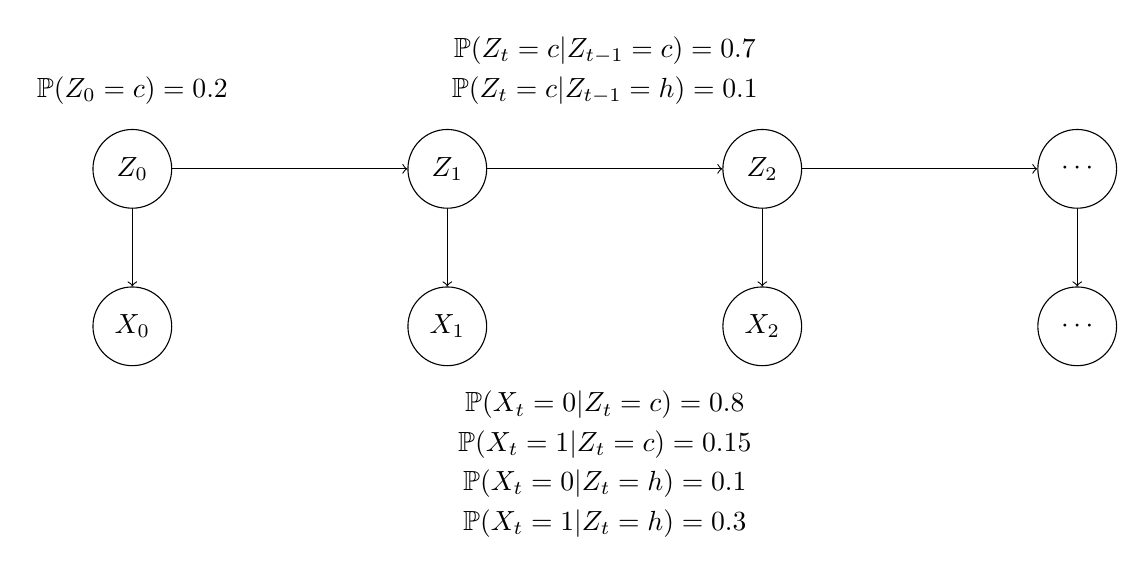
\begin{tikzpicture}
        \node[circle, draw, minimum size=1cm] (Z0) at (0,0) {\(Z_0\)};
        \node[circle, draw, minimum size=1cm] (X0) at (0,-2) {\(X_0\)};
        \node[circle, draw, minimum size=1cm] (Z1) at (4,0) {\(Z_1\)};
        \node[circle, draw, minimum size=1cm] (X1) at (4,-2) {\(X_1\)};
        \node[circle, draw, minimum size=1cm] (Z2) at (8,0) {\(Z_2\)};
        \node[circle, draw, minimum size=1cm] (X2) at (8,-2) {\(X_2\)};
        \node[circle, draw, minimum size=1cm] (Z_inf) at (12,0) {\(\cdots\)};
        \node[circle, draw, minimum size=1cm] (X_inf) at (12,-2) {\(\cdots\)};

        \node (P_Z0) at (0,1) {\(\P(Z_0 = c) = 0.2\)};
        \node (P_Z_c) at (6, 1.5) {\(\P(Z_t = c | Z_{t-1} = c) = 0.7\)};
        \node (P_Z_h) at (6, 1) {\(\P(Z_t = c | Z_{t-1} = h) = 0.1\)};
        \node (P_X0_c) at (6, -3) {\(\P(X_t = 0 | Z_t = c) = 0.8\)};
        \node (P_X1_c) at (6, -3.5) {\(\P(X_t = 1 | Z_t = c) = 0.15\)};
        \node (P_X0_h) at (6, -4) {\(\P(X_t = 0 | Z_t = h) = 0.1\)};
        \node (P_X1_h) at (6, -4.5) {\(\P(X_t = 1 | Z_t = h) = 0.3\)};

        \draw[->] (Z0) -- (Z1);
        \draw[->] (Z1) -- (Z2);
        \draw[->] (Z2) -- (Z_inf);
        \draw[->] (Z0) -- (X0);
        \draw[->] (Z1) -- (X1);
        \draw[->] (Z2) -- (X2);
        \draw[->] (Z_inf) -- (X_inf);
    \end{tikzpicture}
    \caption{HMM with Probabilities Example}
    \label{fig:hmm_probs_viterbi}
\end{figure}

\subsection{Example} \label{sec:viterbi_example}

Suppose on a 4-day interval, we have eaten the following numbers of ice creams:

\begin{verbatim}
    X = [0, 1, 2, 1]
\end{verbatim}

We will consider the numbers sequentially. 

\subsubsection{Day 0}

On day 0, the number of ice cream we have eaten is 0, and we would like to compute the most likely hidden state on day 0. This motivates the use of \textit{Bayes' Rule}:
\begin{align*}
    z_0 &= \arg \max_z \P(Z_0 = z | X_0 = 0) \\
    &= \arg \max_z \frac{\P(X_0 = 0|Z_0 = z) \P(Z_0 = z)}{\P(X_0 = 0)} \\
    &= \arg \max_z \P(X_0 = 0|Z_0 = z) \P(Z_0 = z).
\end{align*}

This separates into 2 cases:
\[\P(X_0=0 | Z_0 = c) \P(Z_0 = c) = 0.8 \cdot 0.2 = 0.16; \hspace{2cm} \P(X_0=0 | Z_0 = h) \P(Z_0 = h) = 0.1 \cdot 0.8 = 0.08.\]
Therefore, it is more likely that \(z_0 = c\) than \(z_0 = h\).

\subsubsection{Day 1}

On day 1, we have eaten 1 ice cream. Note that the probability of interest at this time step is the following, given the conditional independence relationships in the HMM:
\begin{align*}
    \P(Z_0, Z_1 | X_0 = 0, X_1 = 1) &= \frac{\P(X_0 = 0, X_1 = 1, Z_0, Z_1)}{\P(X_0 = 0, X_1 = 1)} \\
    &\propto \P(X_0 = 0, X_1 = 1, Z_0, Z_1) \\
    &= \P(Z_1, X_0 = 0, X_1 = 1 | Z_0) \P(Z_0) \\
    &= \P(Z_0) \P(X_0 = 0, X_1 = 0 | Z_0, Z_1) \P(Z_1 | Z_0) \\
    &= \P(Z_0)\P(X_0 = 0 | Z_0) \P(Z_1|Z_0)  \P(X_1 = 1 | Z_1).
\end{align*}

In the last line of the above equation, note that the first two terms come from the previous time step \(t = 0\), the third term is the transition probability, and the last term is the emission probability. Since the first two terms do not contain \(Z_1\), we should always choose the most likely hidden state from the previous time step, suggesting a dynamic programming approach. With \(Z_0 = c\), we can compute day 1 as follows:
\begin{align*}
    \P(z_0, Z_1 = c | X_0 = 0, X_1 = 1) &\propto \P(z_0)\P(X_0 = 0 | z_0)\P(Z_1 = c | z_0) \P(X_1 = 1 | Z_1 = c) \\
    &= 0.16 \cdot 0.7 \cdot 0.15 \\
    &= 0.0168; \\
    \P(z_0, Z_1 = c | X_0 = 0, X_1 = 1) &\propto \P(z_0)\P(X_0 = 0 | z_0)\P(Z_1 = h | z_0) \P(X_1 = 1 | Z_1 = h) \\
    &= 0.16 \cdot 0.3 \cdot 0.3 \\
    &= 0.0144.
\end{align*}
Therefore, it is more likely that \(z_1 = c\) than \(z_1 = h\).

\subsubsection{Day 2}

We will use the same technique to compute the probability of day 2:
\begin{align*}
    \P(z_0, z_1, Z_2 = c | X_0 = 0, X_1 = 1, X_2 = 2) &\propto \P(z_0, z_1|x_0, x_1) \P(Z_2 = c |z_1) \P(x_2 | Z_2 = c) \\
    &= 0.0168 \cdot 0.7 \cdot 0.05 \\
    &= 0.000588; \\
    \P(z_0, z_1, Z_2 = h | X_0 = 0, X_1 = 1, X_2 = 2) &\propto \P(z_0, z_1|x_0, x_1) \P(Z_2 = h |z_1) \P(x_2 | Z_2 = h) \\
    &= 0.0168 \cdot 0.3 \cdot 0.6 \\
    &= 0.003024.
\end{align*}
Therefore, it is more likely that \(z_2 = h\) than \(z_2 = c\).

\subsubsection{Day 3}

We will use the same technique to compute the probability of day 3:
\begin{align*}
    \P(z_0, z_1, z_2, Z_3 = c | X_0 = 0, X_1 = 1, X_2 = 2, X_3 = 1) &\propto \P(z_0, z_1, z_2|x_0, x_1, x_2) \P(Z_3 = c |z_2) \P(x_3 | Z_3 = c) \\
    &= 0.003024 \cdot 0.1 \cdot 0.15 \\
    &= 0.00004536; \\
    \P(z_0, z_1, z_2, Z_3 = h | X_0 = 0, X_1 = 1, X_2 = 2, X_3 = 1) &\propto \P(z_0, z_1, z_2|x_0, x_1, x_2) \P(Z_3 = h |z_2) \P(x_3 | Z_3 = h) \\
    &= 0.003024 \cdot 0.9 \cdot 0.3 \\
    &= 0.00081648.
\end{align*}
Therefore, it is more likely that \(z_3 = h\) than \(z_3 = c\).

\subsubsection{Conclusion}

Overall, given the observations

\begin{verbatim}
    X = [0, 1, 2, 1]
\end{verbatim}

the most likely sequence of hidden states computed using the \textit{Viterbi} algorithm is

\begin{verbatim}
    Z = [c, c, h, h]
\end{verbatim}

\subsection{Implementation}

The \textit{Viterbi} algorithm is implemented in the \texttt{viterbi.py} file. The algorithm is split into two parts: \texttt{viterbi\_base} and \texttt{viterbi\_step}. The main function \texttt{viterbi} uses the split functions to execute the algorithm and compute the most likely sequence of hidden states. The main function has the following signature:

\begin{minted}{python}
    viterbi(hmm: HiddenMarkovModel, observations: list) -> list
\end{minted}

Running code for the example illustrated above, we would get the outputs

\begin{minted}{python}
    >>> hmm = read_hmm_from_txt('hmm_ex.txt')
    >>> viterbi(hmm, [0, 1, 2, 1])
    ['c', 'c', 'h', 'h']
\end{minted}

which match our manual calculations above.

\subsection{Notes}

\subsubsection{Normalization}

From our manual calculations above in \textit{Chapter \ref{sec:viterbi_example}}, we notice that the computed probabilities got exponentially smaller as the number of time steps increased. This quickly leads to numerical stability and underflow issues. To prevent this, the Python implementation normalizes the returned probabilities at each time step so that the probabilities stay at a manageable level.

\subsubsection{\texttt{HiddenMarkovModel.time\_step}}

Note that the \texttt{HiddenMarkovModel} has an attribute called \texttt{time\_step} that is supposed to specify the number of states in the HMM. This attribute only matters when computing the joint probabilities of the variables in the HMM using the \texttt{\_\_call\_\_} method or the \textit{Variable Elimination} algorithm. The \textit{Viterbi} algorithm only uses the \texttt{initial\_distribution}, \texttt{transition\_distribution}, and \texttt{emission\_distribution} attributes of the HMM, and thus the \texttt{viterbi} function described above can compute the most likely sequence of hidden states of any length under the given HMM setup. The length of the returned sequence is solely determined by the length of the input observations.

\pagebreak

\section{The Forward-Backward Algorithm}

\subsection{Motivation}

In the previous section where we explored the \textit{Viterbi} algorithm, the problem we were interested in solving was to find the most likely sequence of hidden states given a sequence of observations. In this section, we explore the case where we don't care the entire sequence of hidden states, but only the probability distribution of the hidden state at a certain time step \(t\). As mentioned in \textit{Chapter \ref{sec:hmm_intro}}, the following types of tasks are generally of interest to us:

\begin{enumerate}
    \item \textbf{Filtering} -- \(\P(Z_T | \vec x)\). Compute the probability of the hidden state at \textit{current} time \(T\) based on all observations;
    \item \textbf{Smoothing} -- \(\P(Z_t | \vec x)\) for \(0 \leq t < T\). Compute the probability of the hidden state at \textit{past} time \(t\) based on all observations;
    \item \textbf{Prediction} -- \(\P(Z_t | \vec x)\) for \(t > T\). Compute the probability of the hidden state at \textit{future} time \(t\) based on all observations;
    \item \textbf{Most Likely Sequence} -- \(\arg \max_{\vec z} \P(\vec z | \vec x)\). Compute the most likely sequence of hidden states given the observations.
\end{enumerate}

In this chapter, we will explore algorithms that solve problems 1 and 2. Below is the example HMM again for reference.

\begin{figure}[htbp]
    \centering
    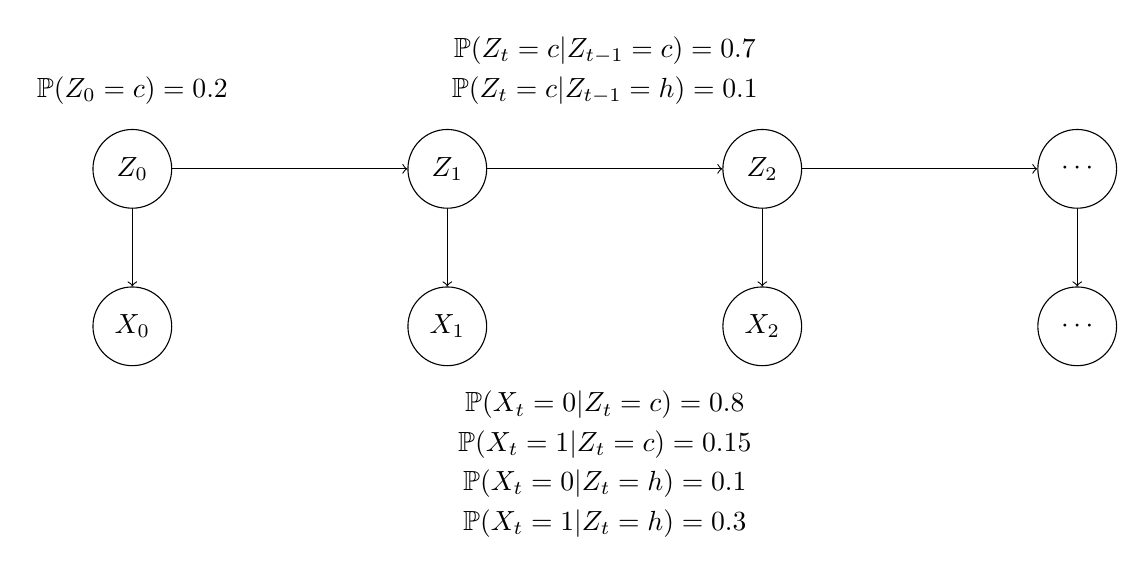
\begin{tikzpicture}
        \node[circle, draw, minimum size=1cm] (Z0) at (0,0) {\(Z_0\)};
        \node[circle, draw, minimum size=1cm] (X0) at (0,-2) {\(X_0\)};
        \node[circle, draw, minimum size=1cm] (Z1) at (4,0) {\(Z_1\)};
        \node[circle, draw, minimum size=1cm] (X1) at (4,-2) {\(X_1\)};
        \node[circle, draw, minimum size=1cm] (Z2) at (8,0) {\(Z_2\)};
        \node[circle, draw, minimum size=1cm] (X2) at (8,-2) {\(X_2\)};
        \node[circle, draw, minimum size=1cm] (Z_inf) at (12,0) {\(\cdots\)};
        \node[circle, draw, minimum size=1cm] (X_inf) at (12,-2) {\(\cdots\)};

        \node (P_Z0) at (0,1) {\(\P(Z_0 = c) = 0.2\)};
        \node (P_Z_c) at (6, 1.5) {\(\P(Z_t = c | Z_{t-1} = c) = 0.7\)};
        \node (P_Z_h) at (6, 1) {\(\P(Z_t = c | Z_{t-1} = h) = 0.1\)};
        \node (P_X0_c) at (6, -3) {\(\P(X_t = 0 | Z_t = c) = 0.8\)};
        \node (P_X1_c) at (6, -3.5) {\(\P(X_t = 1 | Z_t = c) = 0.15\)};
        \node (P_X0_h) at (6, -4) {\(\P(X_t = 0 | Z_t = h) = 0.1\)};
        \node (P_X1_h) at (6, -4.5) {\(\P(X_t = 1 | Z_t = h) = 0.3\)};

        \draw[->] (Z0) -- (Z1);
        \draw[->] (Z1) -- (Z2);
        \draw[->] (Z2) -- (Z_inf);
        \draw[->] (Z0) -- (X0);
        \draw[->] (Z1) -- (X1);
        \draw[->] (Z2) -- (X2);
        \draw[->] (Z_inf) -- (X_inf);
    \end{tikzpicture}
    \caption{HMM with Probabilities Example}
    \label{fig:hmm_probs_forward_backward}
\end{figure}

\subsection{The Forward Algorithm} \label{sec:forward_algorithm}

\subsubsection{Theory}

Suppose we have observations

\begin{verbatim}
    X = [x0 = 0, x1 = 1, x2 = 2, x3 = 1, x4 = 1, x5 = 2, x6 = 0]
\end{verbatim}

Since we have 7 observations from \(x_0\) to \(x_6\), we define \(T = 6\) as the last time step of the observations. For \(t\in \{0, 1, \cdots, T\}\), we define the \textit{filtered marginal} \(\alpha_t\) as
\[\alpha_t(j) = \P(Z_t = j | x_{0:t}).\]
In other words, \(\alpha_t(j)\) is the probability that the hidden state at time \(t\) is \(j\) given its current and preceding observations. Note that for the base case \(t=0\), we have
\begin{align*}
    \alpha_0(j) &= \P(Z_0 = j | x_0) \\
    &= \frac{\P(x_0 | Z_0 = j) \P(Z_0 = j)}{\P(x_0)} \\
    &\propto \P(x_0 | Z_0 = j) \P(Z_0 = j) \\
    &= \pi(j) \phi(j, x_0),
\end{align*}
which is the product of the initial probability and the emission probability of the HMM.

Now, the \textit{Forward} algorithm comes into play to compute the filtered marginals \(\alpha_t\) for \(t > 0\). This algorithm has two steps: A \textit{Prediction} step and a \textit{Update} step. For \(t > 0\), by the \textit{Law of Total Probability}, the prediction step runs as follows:
\begin{align*}
    \tau_t(j) &= \P(Z_t = j | x_{0:t-1}) \\
    &= \sum_i \P(Z_t = j | Z_{t-1} = i, x_{0:t-1})\P(Z_{t-1} = i | x_{0:t-1}) \\
    &= \sum_i \P(Z_t = j | Z_{t-1} = i) \P(Z_{t-1} = i | x_{0:t-1}) \\
    &= \sum_i \psi(i, j) \alpha_{t-1}(i).
\end{align*}
With prediction \(\tau_t\), we can update the filtered marginal \(\alpha_t\) as follows:
\begin{align*}
    \alpha_t(j) &= \P(Z_t = j | x_{0:t}) \\
    &= \P(Z_t = j | x_{0:t-1}, x_t) \\
    &\propto \P(x_t | Z_t = j, x_{0:t-1}) \P(Z_t = j | x_{0:t-1}) \\
    &= \P(x_t | Z_t = j) \P(Z_t = j | x_{0:t-1}) \\
    &= \phi(j, x_t) \tau_t(j).
\end{align*}
Therefore, with the above recurrence relation, we can compute the filtered marginals \(\alpha_t\) at any time step \(t\) for \(t\in \{0, 1, \cdots, T\}\) given observations \(x_{0:T}\). Now, notice our objective probability for the \textit{Filtering} task
\[\P(Z_T | \vec x) = \P(Z_T | x_{0:T}) = \alpha_T,\]
which is exactly the filtered marginal at the last time step \(T\). Therefore, the \textit{Filtering} task can be computed by a pass of the \textit{Forward} algorithm.

\subsubsection{Implementation}

The \textit{Forward} algorithm is implemented in the \texttt{forward\_backward.py} file in the \texttt{forward} function, which has the following signature:

\begin{minted}{python}
    forward(hmm: HiddenMarkovModel, observations: list, t: int=0) -> dict
\end{minted}

This function takes in a \texttt{HiddenMarkovModel} instance, a list of observations, and a time step \(t\), and it outputs the filtered marginal \(\alpha_t\) at time step \(t\). To run the \textit{Filtering} task, a function called \texttt{filtering} is provided that has the following signature:

\begin{minted}{python}
    filtering(hmm: HiddenMarkovModel, observations: list) -> dict
\end{minted}

This function basically calls \texttt{forward} with \(t = T\), where \(T\) is the length of the observations minus 1.

With the HMM defined in \textit{Figure \ref{fig:hmm_probs_forward_backward}}, we can run code as follows:

\begin{minted}{python}
    >>> hmm = read_hmm_from_txt('hmm_ex.txt')
    >>> filtering(hmm, [0, 1, 2, 1, 1, 2, 0])
    {'h': 0.5070962425796098, 'c': 0.4929037574203903}
\end{minted}

The outputs tell us that it is almost equally likely that day 6 is either hot or cold based on the observations.

\subsection{The Forward-Backward Algorithm} \label{sec:forward_backward_algorithm}

\end{document}